\documentclass[12pt, twoside]{article}
\usepackage[francais]{babel}
\usepackage[T1]{fontenc}
\usepackage[latin1]{inputenc}
\usepackage[left=7mm, right=7mm, top=7mm, bottom=7mm]{geometry}
\usepackage{float}
\usepackage{graphicx}
\usepackage{array}
\usepackage{multirow}
\usepackage{amsmath,amssymb,mathrsfs} 
\usepackage{soul}
\usepackage{textcomp}
\usepackage{eurosym}
 \usepackage{variations}
\usepackage{tabvar} 

\begin{document}

\begin{center}
\textbf{Constructions}
\end{center}


\ul{\textbf{Exercice 1:}} Pour chacun des triangles ci-dessous, dire s'il s'agit
d'une hauteur, d'une m�diatrice, d'une m�diane ou d'une bissectrice.


\begin{tabular}{cc}
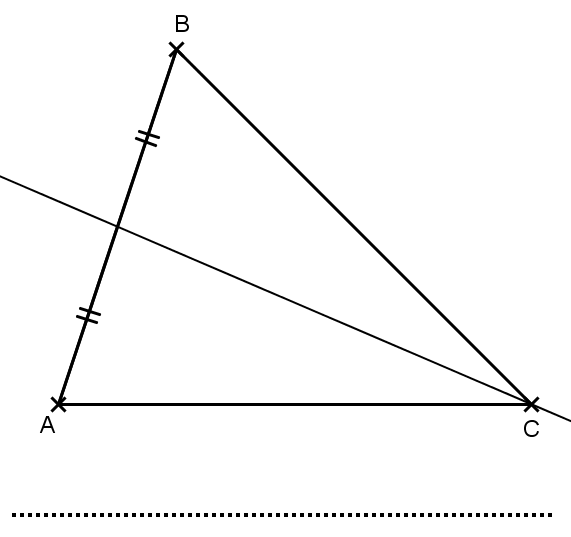
\includegraphics[width=5cm]{images/ex11.png} \qquad \qquad \qquad
&
\qquad \qquad \qquad 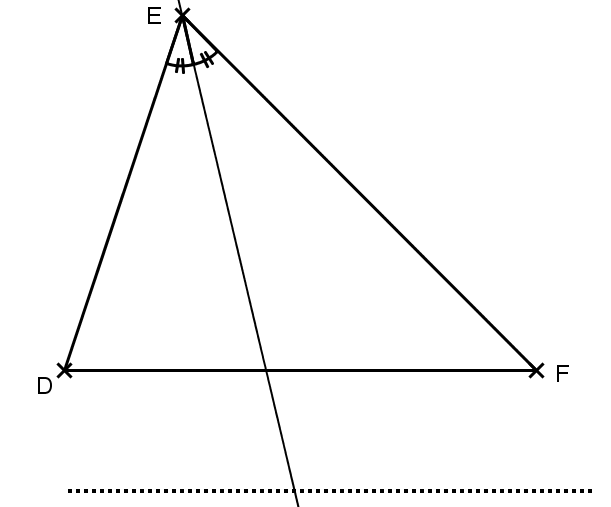
\includegraphics[width=5cm]{images/ex12.png}\\


\qquad \qquad \qquad 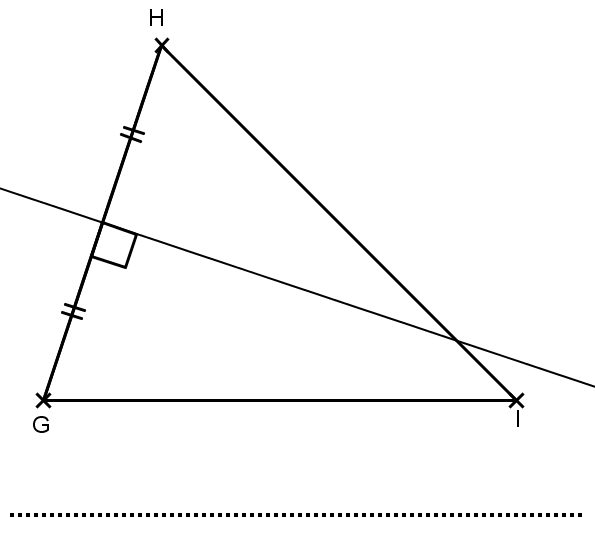
\includegraphics[width=5cm]{images/ex13.png} \qquad
\qquad \qquad &
\qquad \qquad \qquad 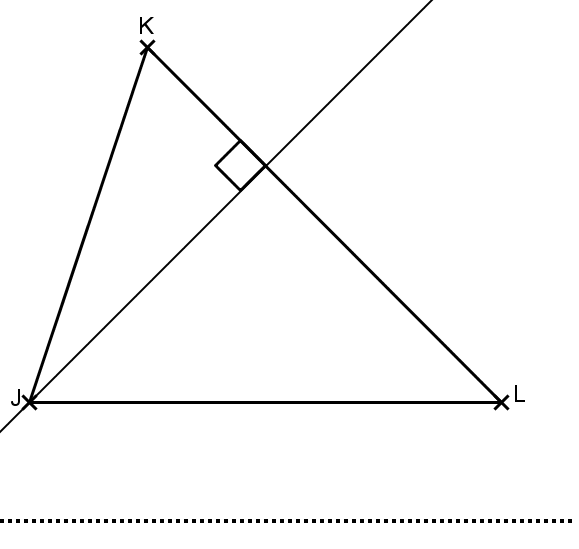
\includegraphics[width=5cm]{images/ex14.png} \\

\end{tabular}


\bigskip

\bigskip



\begin{tabular}{cc}
\begin{minipage}{9cm}
\ul{\textbf{Exercice 2:}} 

\begin{enumerate}
  \item Construire un triangle ABC quelconque. \qquad \qquad \qquad
  \item  Tracer la m�diane issue de A  
\item Tracer la m�diane issue de B.
\item Tracer la m�diane issue de C.
 \item Que remarque-t-on?
\end{enumerate} 
\end{minipage}
&

\begin{minipage}{9cm}
\ul{\textbf{Exercice 3:}} 

\begin{enumerate}
\item Construire un triangle ABC quelconque.
\item  Tracer la m�diatrice de [AB].  
\item Tracer la m�ditrice de [AC].
\item Tracer la m�diatrice de [BC]
\item Que remarque-t-on?
\end{enumerate} 
\end{minipage}
\end{tabular}


\bigskip

\bigskip


\ul{\textbf{Exercice 4:}} Construire les cercles circonscrits des triangles
suivants:



\begin{tabular}{cc}

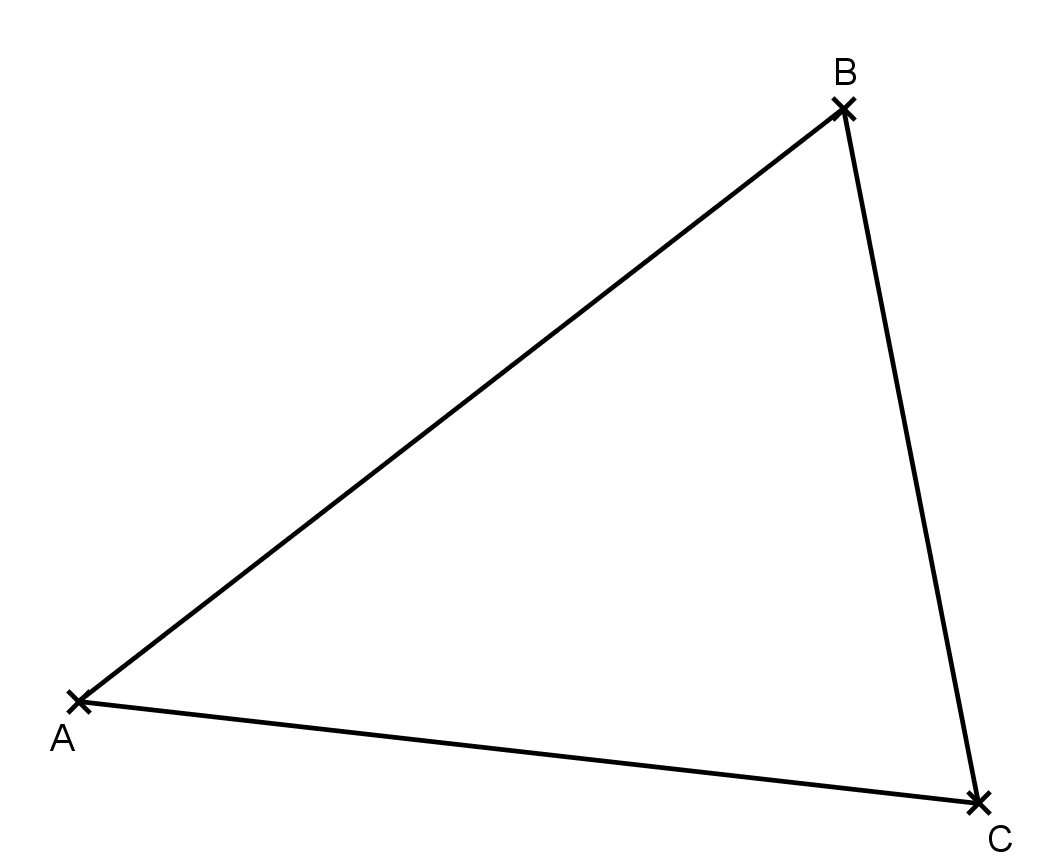
\includegraphics[width=6cm]{images/ex41.png} \qquad \qquad \qquad

&

\qquad \qquad 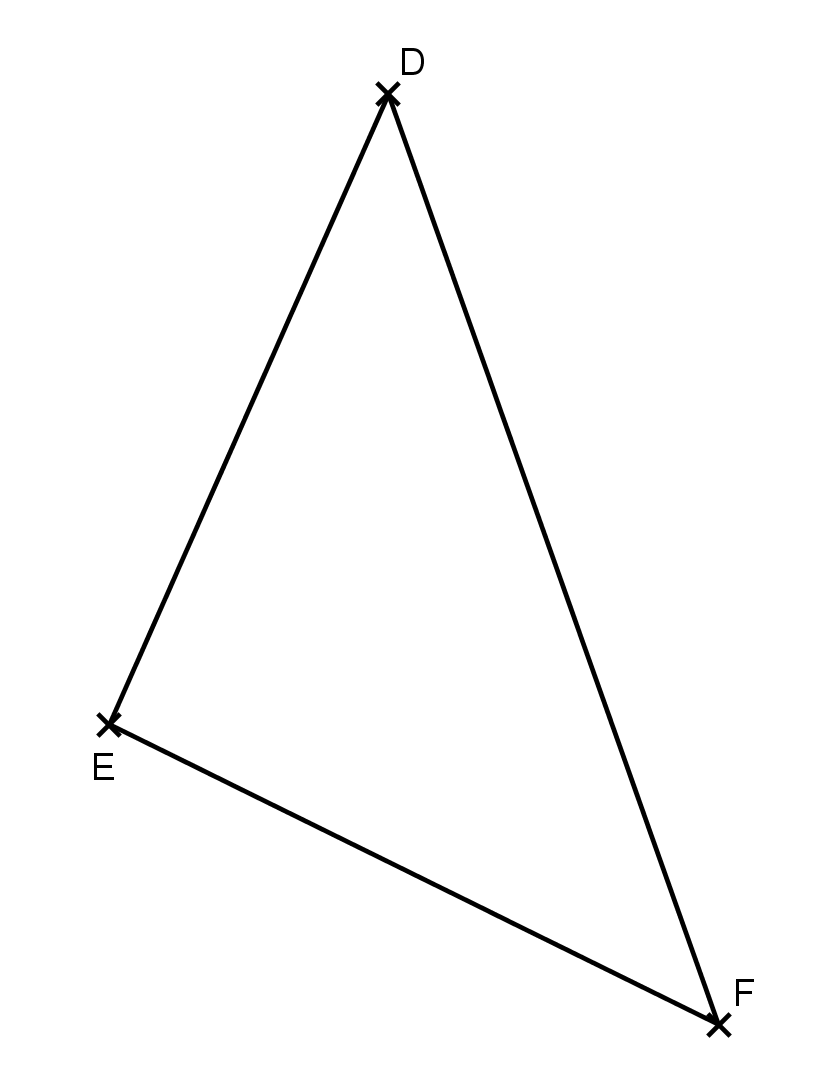
\includegraphics[width=6cm]{images/ex42.png} \\
\end{tabular}

\end{document}
